\section{切空间把``方向''还给弯曲空间}
\label{sec:12-Real-Analysis-Support/08-Manifold-Basics/02}

在平面上，``从 \(p\) 出发沿 \(v\) 走一步''就是写下 \(p+tv\)。加法是全局的，不附带任何前提。现在把脚站到单位球面上，站在纬度 \(45^{\circ}\) 的某点 \(p\)，说一句``往东走一小步''。你想照旧写 \(p+tv\)，可是无论 \(v\) 取哪个三维向量，只要 \(t\neq 0\)，\(p+tv\) 就掉出球面了——球面对向量加法不封闭。

麻烦不止球面有。数据流形、参数空间、机器人的位形空间，都没有免费的加法。而微积分的第一步永远是线性化，线性化又必须先有``方向''才能谈``沿这个方向的变化率''。方向这个词要是救不回来，弯曲空间上的微积分就没有地基。

\begin{center}
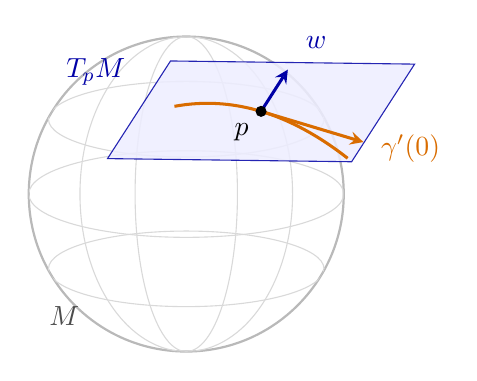
\begin{tikzpicture}[>=stealth,scale=1.0]
% 球面轮廓
\draw[gray!55,thick] (0,0) circle (2);
% 经纬网（手工二维投影）
\begin{scope}
  \clip (0,0) circle (2);
  \draw[gray!30] (0,0) ellipse (2 and 0.55);
  \draw[gray!30] (0,0.95) ellipse (1.75 and 0.48);
  \draw[gray!30] (0,-0.95) ellipse (1.75 and 0.48);
  \draw[gray!30] (0,0) ellipse (0.65 and 2);
  \draw[gray!30] (0,0) ellipse (1.35 and 2);
\end{scope}
% 切点 p
\coordinate (P) at (0.95,1.05);
% 切平面（手工投影成平行四边形）
\draw[blue!65!black,fill=blue!7,opacity=0.85]
  (2.90,1.65) -- (2.10,0.41) -- (-1.00,0.45) -- (-0.20,1.69) -- cycle;
% 曲面上过 p 的一条曲线
\draw[orange!85!black,line width=1.1pt]
  plot[domain=-1.1:1.1,samples=40] ({0.95+\x*1.0},{1.05-0.30*\x-0.22*\x*\x});
% 切向量
\draw[->,line width=1.1pt,orange!85!black] (P) -- ++(1.30,-0.39);
\draw[->,line width=1.1pt,blue!65!black] (P) -- ++(0.34,0.53);
\fill (P) circle (2pt);
\node[below left=1pt] at (P) {\(p\)};
\node[orange!85!black,anchor=west] at (2.35,0.58) {\(\gamma'(0)\)};
\node[blue!65!black] at (1.65,1.92) {\(w\)};
\node[blue!65!black] at (-1.15,1.55) {\(T_{p}M\)};
\node[gray!60!black] at (-1.55,-1.55) {\(M\)};
\end{tikzpicture}
\end{center}

\emph{曲面在 \(p\) 处贴着一张平面，过 \(p\) 的每条曲线在这张平面上留下一个速度向量。}

\subsection{坐标卡能给出速度，可惜每张卡给的不一样}

流形的标准逃生路线是翻到一张卡上去。在 \(p\) 附近用球极投影 \(\varphi\) 把一片球面摊成圆盘，过 \(p\) 的球面曲线 \(\gamma(t)\)（\(\gamma(0)=p\)）就变成平面上一条普通曲线 \(\varphi\circ\gamma\)，它在 \(t=0\) 处的速度 \((\varphi\circ\gamma)'(0)\) 是货真价实的二维向量。方向似乎回来了。

换一张卡，它又跑了。改用经纬度参数化，同一条曲线的速度向量数值完全不同。两张卡之间隔着转移映射 \(\psi\circ\varphi^{-1}\)，链式法则给出

\[
(\psi\circ\gamma)'(0)=J\,(\varphi\circ\gamma)'(0),
\qquad J=D(\psi\circ\varphi^{-1})\big|_{\varphi(p)},
\]

两个速度向量差一个可逆矩阵。按上一节立下的纪律，随卡而变的数值不能算流形上的对象。但这里的变化方式是被 \(J\) 完全规定的——这恰好是纪律允许的那一类。线索就在这里。

\subsection{把一阶行为相同的曲线捆在一起，方向就成了对象}

既然单张卡给出的向量不唯一，那就别追着某一个数值不放，改去问：哪些曲线在 \(p\) 处``走得一样快、一样的方向''。

\begin{definition}[切向量]
设 \(\gamma,\sigma\) 是过 \(p\) 的光滑曲线，\(\gamma(0)=\sigma(0)=p\)。若存在一张含 \(p\) 的坐标卡 \((U,\varphi)\) 使 \((\varphi\circ\gamma)'(0)=(\varphi\circ\sigma)'(0)\)，就称二者在 \(p\) 处一阶等价。一个等价类叫做 \(M\) 在 \(p\) 处的一个切向量，全体切向量的集合记作 \(T_{p}M\)。
\end{definition}

定义里藏着一处需要兑现的承诺：``存在一张卡''能不能升级成``所有卡''。能。若在 \(\varphi\) 下两条曲线速度相同，那么在任一张 \(\psi\) 下，两者的速度同时被同一个 \(J\) 左乘，相等关系原样保留；\(J\) 可逆，所以反过来也成立。条件对账：只用到转移映射光滑（保证 \(J\) 存在）与可逆（保证等价关系不被压缩），二者都写在流形的定义里。等价类的划分因此与卡无关。

固定一张卡，映射 \([\gamma]\mapsto(\varphi\circ\gamma)'(0)\) 是 \(T_{p}M\) 与 \(\R^{d}\) 之间的一一对应——给定任一 \(u\in\R^{d}\)，曲线 \(t\mapsto\varphi^{-1}(\varphi(p)+tu)\) 就是一个代表元。把 \(\R^{d}\) 的加法与数乘搬回来，\(T_{p}M\) 成为 \(d\) 维向量空间。搬运的结果不依赖卡的选择，因为不同卡之间差的 \(J\) 是线性同构。第 \(i\) 条坐标曲线的速度类记作 \(\partial/\partial x^{i}|_{p}\)，它们构成一组基。

\subsection{切空间是平的，弯的始终是流形}

这个构造有个值得停下来看的后果：\(T_{p}M\) 永远是向量空间，永远平直。弯曲属于 \(M\)，不属于它的任何一个切空间。

对嵌在 \(\R^{3}\) 中的球面，切空间能直接算出来。球面上的曲线满足 \(\ip{\gamma(t)}{\gamma(t)}=1\)，两边求导得 \(2\ip{\gamma'(t)}{\gamma(t)}=0\)，在 \(t=0\) 处即 \(\ip{\gamma'(0)}{p}=0\)。反过来，任给与 \(p\) 正交的 \(v\)，曲线 \(t\mapsto\cos(t)\,p+\sin(t)\,v/\norm{v}\) 留在球面上且速度方向为 \(v\)。两边合起来，

\[
T_{p}S^{2}=\set{v\in\R^{3}:\ip{v}{p}=0}.
\]

北极处这是水平的 \(xy\) 平面，赤道上某点处它是竖直的。每一点手上都有一张平面，各点的平面朝向不同——弯曲正是藏在``朝向如何随点变化''里，而不在任何单张平面内部。上面那张图画的就是这件事：平面贴着曲面，曲面随即从两侧弯开。

\subsection{切向量属于点，位移属于空间}

有两处混淆几乎人人踩过一次，值得说破。

第一处：\(v\in T_{p}S^{2}\) 是 \(\R^{3}\) 里的向量，但 \(p+v\) 一般不在球面上。切空间告诉你此刻可以朝哪些方向出发，不告诉你出发以后路怎么拐。``沿 \(v\) 走一步''需要流形自己的运动规则，那是下一节测地线的事。

第二处：切平面与球面是一阶贴合，二阶就分家了。切空间对曲率一无所知，这跟 Taylor 展开里一阶项管不着二阶项是同一回事。

顺着第一处再往前一点：在 \(\R^{n}\) 里我们习惯把切向量和位移混为一谈，是因为那里的空间本身就直，把 \(p\) 处的向量平移到 \(q\) 处不费力气。弯曲流形上没有这种便利，每一点有自己的切空间，\(T_{p}M\) 与 \(T_{q}M\) 之间不存在天然的对照表。要在它们之间搬运向量，得额外指定一个联络，由它规定沿路径运输时向量该怎么转。本单元不展开这个结构，但知道它是额外加的，比误以为它自带要好。

\subsection{``局部线性''这句口号的精确版本就是切空间}

降维方法反复讲的``数据在局部近似一个低维线性块''，翻成这里的语言只有一句：那个线性块是切空间。

设生成映射 \(F:\mathcal{A}\to\mathcal{X}\) 把少量内在自由度送成观测空间里的数据点。在 \(a\) 处展开，

\[
F(a+h)=F(a)+dF_{a}h+o(\norm{h}),
\]

其中 \(dF_{a}:T_{a}\mathcal{A}\to T_{F(a)}\mathcal{X}\) 是 \(F\) 的微分——它把一个切向量的代表曲线 \(\gamma\) 送成 \(F\circ\gamma\)，取后者的速度类。像集在 \(F(a)\) 附近被 \(dF_{a}(T_{a}\mathcal{A})\) 一阶逼近，这就是那个线性块。全局的弯曲则来自两件事：\(dF_{a}\) 随 \(a\) 变化，以及 \(F\) 未必单射。自编码器的隐空间大致扮演 \(\mathcal{A}\) 的角色，解码器扮演 \(F\)——这是类比，不是定理，因为没人保证学到的解码器处处满秩。

而 \(dF_{a}\) 在某点掉秩，正是这套语言里``奇点''的样子：那里的局部自由度比别处少，切空间的维数塌下去一截，基于近邻图的方法在那种地方最容易把不该相连的点连起来。

\subsection{有了方向，还欠一把尺}

到这里，弯曲空间上已经有了方向：每点一个 \(d\) 维向量空间，映射在其间诱导线性映射，链式法则 \(d(G\circ F)_{p}=dG_{F(p)}\circ dF_{p}\) 逐字照搬，不需要为弯曲添加任何修正项。

但切空间只是向量空间，不是内积空间。两个切向量之间的夹角是多少、一个切向量有多长、一条曲线走了多远，这些问题目前一个也答不了——向量空间的公理里根本没有长度。下一节\hyperref[sec:12-Real-Analysis-Support/08-Manifold-Basics/03]{``黎曼度量让弯曲空间有长度''}要做的，就是在每个切空间上装一个内积，并且说清楚这把尺是外加的选择，不是流形自带的事实。
